%#-*- coding: utf-8 -*-
\documentclass{ctexart}
%
%页眉页脚
\usepackage{geometry}
\geometry{left=2.5cm,right=2.5cm,top=2.5cm,bottom=2.5cm}
\usepackage{xcolor}
\usepackage{graphicx}
\usepackage{amsmath}
\usepackage{url}
\usepackage{enumerate}
\usepackage{subfigure}
\usepackage{listings}
\usepackage[colorlinks,linkcolor=black]{hyperref}%书签
\usepackage{fancyhdr}

\fancyhead[R]{\thepage}%这是奇数页右页眉、偶数页左页眉
\fancyhead[L]{}
\chead{全球导航卫星系统基础}%这是中间页眉
\pagestyle{fancy}
\lstset{
    extendedchars=false, %解决代码跨页时,章节标题,页眉等汉字不显示的问题
    xleftmargin=1.5em,xrightmargin=1.5em, aboveskip=1em, %设置边距
    language=Matlab,
    basicstyle = \footnotesize,
    breaklines,
    captionpos = t,
    commentstyle = \color[rgb]{0,0.5,0},
    frameshape = {RYRYNYYYY}{yny}{yny}{RYRYNYYYY},
    keywordstyle = \color{blue}\bfseries,
    numbers = left,
    numberstyle = \tiny\color[rgb]{0.5,0.5,0.5},
    showstringspaces = false,
    stringstyle = \color[rgb]{0.58,0,0.82},
    tabsize = 4,
    title = \lstname
}
%中文
\usepackage{xeCJK}
%字体设置
\usepackage{enumitem}
\usepackage{indentfirst}
\setlength{\parindent}{2em}%首行缩进
\renewcommand\thesubsection{\alph{subsection}}
\renewcommand\thesubsubsection{\alph{subsubsection}}
\CTEXsetup[format={\Large\bfseries}]{section}

\title{AVL树$\rightarrow$红黑树问题}
\author{聂浩~~无31~~ 2013011280}
\date{\today}
\begin{document}
\maketitle
\section{实验内容}
在Windows的虚拟内存管理中,将VAD组织成AVL树。VAD树是一种平衡二叉树。

红黑树也是一种自平衡二叉查找树,在Linux 2.6及其以后版本的内核中,采用红黑树来维护内存块。

请尝试参考Linux源代码将WRK源代码中的VAD树由AVL树替换成红黑树。

\section{实验思路}
红黑树与AVL的查找基本是一致的,不需要太多的修改。

插入与删除函数通过对linux(v4.4-rc6)与WRK1.2的分析。利用用linux的红黑树代码替换WRK中的AVL管理。
\subsection{Linux中的红黑树}
Linux中,虚拟内存管理的VAD由红黑树实现。

红黑树是一种在插入或删除节点是都需要维持平衡的二叉查找树,且每个节点都具有颜色属性:
\begin{enumerate}
    \item{一个结点要么是红色的,要么是黑色的。}
    \item{根结点是黑色的。}
    \item{如果一个结点是红色的,那么它的子结点必须是黑色的,也就是说在沿着从根结点出发的任何路径上都不会出现两个连续的红色结点。}
    \item{从一个结点到一个NULL指针的每条路径上必须包含相同数目的黑色结点。}
\end{enumerate}

本次实验使用Linux Kernel 4.4-rc6版本。

linux内核源代码中,红黑树的定义在三个地方,分别是
\begin{itemize}
    \item{include/linux/rbtree.h}
    \item{include/linux/rbtree\_augmented.h}
    \item{lib/rbtree.c}
\end{itemize}

其中红黑树节点的定义为:
\begin{lstlisting}[language=C]

struct rb_node {
	unsigned long  __rb_parent_color;
	struct rb_node *rb_right;
	struct rb_node *rb_left;
} __attribute__((aligned(sizeof(long))));
    /* The alignment might seem pointless, but allegedly CRIS needs it */

struct rb_root {
	struct rb_node *rb_node;
};
\end{lstlisting}

有意思的是,这里使用了\_\_attribute\_\_((aligned(sizeof(long)))),使得结构体进行4字节大小对齐(32位系统),因此地址最低两位始终是00,linux使用其中的最低一位表示红黑树节点的颜色。

基于此linux定义了一些基本操作(在rbtree\_augmented.c中):

\begin{lstlisting}[language=C]
\\在rbtree.h中
#define rb_parent(r)   ((struct rb_node *)((r)->__rb_parent_color & ~3))
\\在rbtree_augmented.c
#define	RB_RED		0
#define	RB_BLACK	1

#define __rb_parent(pc)    ((struct rb_node *)(pc & ~3))

#define __rb_color(pc)     ((pc) & 1)
#define __rb_is_black(pc)  __rb_color(pc)
#define __rb_is_red(pc)    (!__rb_color(pc))
#define rb_color(rb)       __rb_color((rb)->__rb_parent_color)
#define rb_is_red(rb)      __rb_is_red((rb)->__rb_parent_color)
#define rb_is_black(rb)    __rb_is_black((rb)->__rb_parent_color)

static inline void rb_set_parent(struct rb_node *rb, struct rb_node *p)
{
	rb->__rb_parent_color = rb_color(rb) | (unsigned long)p;
}
//设置父节点的同时设置自己的颜色
static inline void rb_set_parent_color(struct rb_node *rb,
				       struct rb_node *p, int color)
{
	rb->__rb_parent_color = (unsigned long)p | color;
}

static inline void
__rb_change_child(struct rb_node *old, struct rb_node *new,
		  struct rb_node *parent, struct rb_root *root)
{
	if (parent) {
		if (parent->rb_left == old)
			WRITE_ONCE(parent->rb_left, new);
            \\WRITE_ONCE(a,b)=>a=b;
		else
			WRITE_ONCE(parent->rb_right, new);
	} else
		WRITE_ONCE(root->rb_node, new);
}
\\在rbtree.c中,为旋转做准备
static inline void
__rb_rotate_set_parents(struct rb_node *old, struct rb_node *new,
			struct rb_root *root, int color)
{
	struct rb_node *parent = rb_parent(old);
	new->__rb_parent_color = old->__rb_parent_color;
	rb_set_parent_color(old, new, color);
	__rb_change_child(old, new, parent, root);
}

\end{lstlisting}

linux红黑树的插入:具体调用为rb\_insert\_color,然后再调用内部函数\_\_rb\_insert,这里代码太长不在此处展示,具体代码可见rbtree.c函 数。
需要注意的是,linux的插入函数处理的是节点已经添加在树上后的平衡过程。root指向红黑树的根节点,但是根节点的parent指向NULL。

linux红黑树的删除:具体调用rb\_erase函数,内容如下:

\begin{lstlisting}[language=C]
void rb_erase(struct rb_node *node, struct rb_root *root)
{
	struct rb_node *rebalance;
	rebalance = __rb_erase_augmented(node, root, &dummy_callbacks);
	if (rebalance)
		____rb_erase_color(rebalance, root, dummy_rotate);
}
EXPORT_SYMBOL(rb_erase);
\end{lstlisting}
\_\_rb\_erase\_augmented用于直接删除节点并判断是否破坏了红黑树的性质,在rbtree\_augmented.c中定义,\_\_\_\_rb\_erase\_color用于修复被破坏的红黑树,其代码rbtree.c

除此之外,linux红黑树的实现还有替换rb\_replace\_node,寻找前驱后继等函数,这些红黑树和AVL树没有区别,本实验不需要移植,在这里不再讨论。

\subsection{Windows中的AVL树}
Windows中,虚拟内存管理的VAD是以AVL树的形式管理的。

Windows的虚拟内存管理利用MM\_AVL\_TABLE型变量,其定义在base/ntos/inc/ps.h,
\begin{lstlisting}[language=C]
typedef struct _MM_AVL_TABLE {
	MMADDRESS_NODE  BalancedRoot;
	ULONG_PTR DepthOfTree : 5;
	ULONG_PTR Unused : 3;
#if defined (_WIN64)
	ULONG_PTR NumberGenericTableElements : 56;
#else
	ULONG_PTR NumberGenericTableElements : 24;
#endif
	PVOID NodeHint;
	PVOID NodeFreeHint;
} MM_AVL_TABLE, *PMM_AVL_TABLE;
\end{lstlisting}

其中的BalancedRoot保存了AVL树的根节点信息。NumberGenericTableElements需要在插入和删除节点的时候进行修改。

通过相关资料查询以及对具体源代码的分析可知BalancedRoot的RightChild指向根节点,而根节点的Parent指向BalancedRoot,这里和linux有较大的区别。

MMADDRESS\_NODE的定义在在base/ntos/mm/mi.h里:
\begin{lstlisting}[language=C]
typedef struct _MMADDRESS_NODE {
	union {
		LONG_PTR Balance : 2;
		struct _MMADDRESS_NODE *Parent;
	} u1;
	struct _MMADDRESS_NODE *LeftChild;
	struct _MMADDRESS_NODE *RightChild;
	ULONG_PTR StartingVpn;
	ULONG_PTR EndingVpn;
} MMADDRESS_NODE, *PMMADDRESS_NODE;
\end{lstlisting}

和linux类似的是,Windows也是利用存储的父地址的低两位存储节点的性质(平衡因子),不同的是,Windows的实现方式是联合体。具体实践中发现,该联合体读取时是读出全部4字节,但写入时Balance和Parent需要分开写;红黑树不需要平衡因子,这里利用Balance变量存储颜色。后两个数是存储的页信息,和本实验无关。

Windows中维护AVL树的函数主要有:
\begin{itemize}
    \item{插入MiInsertNode}
    \item{平衡MiRebalanceNode和MiPromoteNode}
    \item{删除MiRemoveNode等等。}
\end{itemize}

对外的接口有MiInsertNode和MiRemoveNode,这也是我们在实验过程中需要保留并重新实现的,它们出现在/base/ntos/mm/addrsup.c中。

\section{实验过程}
为了使用linux中的函数,先定义以下基础操作
\begin{lstlisting}[language=c]

#define rb_black 0
#define rb_red 1

PMMADDRESS_NODE rb_parent(PMMADDRESS_NODE node)
{
	node =SANITIZE_PARENT_NODE(SANITIZE_PARENT_NODE(node)->u1.Parent);
	return node;
}
int rb_color(PMMADDRESS_NODE node)
{
	return node->u1.Balance;
}
int rb_is_red(PMMADDRESS_NODE node)
{
	return node->u1.Balance==rb_red;
}
int rb_is_black(PMMADDRESS_NODE node)
{
	return node->u1.Balance==rb_black;
}
void rb_set_black(PMMADDRESS_NODE node)
{
	node->u1.Balance = rb_black;
}
void rb_set_red(PMMADDRESS_NODE node)
{
	node->u1.Balance = rb_red;
}
void rb_set_parent( PMMADDRESS_NODE rb,PMMADDRESS_NODE p)
{
	rb->u1.Parent =(PMMADDRESS_NODE)(((ULONG_PTR)(p)) + ((ULONG_PTR)(rb->u1.Balance)));
}

void rb_set_color( PMMADDRESS_NODE rb, int color) 
{  
	rb->u1.Balance = color;  
}  

void rb_set_parent_color(PMMADDRESS_NODE rb, PMMADDRESS_NODE p,int color)
{
	rb->u1.Parent =p;
	rb->u1.Balance=color;
}

void __rb_change_child(PMMADDRESS_NODE old, PMMADDRESS_NODE newer,
	PMMADDRESS_NODE parent, PMM_AVL_TABLE root)
{
	if (parent!=&root->BalancedRoot) {
		if (parent->LeftChild== old){
			parent->LeftChild = newer;			
		}
		else
			parent->RightChild = newer;
	} else 
		root->BalancedRoot.RightChild = newer;
}

void __rb_rotate_set_parents(PMMADDRESS_NODE old, PMMADDRESS_NODE newer,PMM_AVL_TABLE root, int color)
{
	PMMADDRESS_NODE parent = rb_parent(old);
	rb_set_color(newer,rb_color(old));
	rb_set_parent(newer,rb_parent(old));
	rb_set_parent_color(old, newer, color);
	__rb_change_child(old, newer, parent, root);
}
\end{lstlisting}

其中SANITIZE\_PARENT\_NODE的定义如下(在ntos/inc/ps.h中)
 \begin{lstlisting}[language=C]
 #define SANITIZE_PARENT_NODE(Parent) ((PMMADDRESS_NODE)(((ULONG_PTR)(Parent)) & ~0x3))
 \end{lstlisting}
 \subsection{插入节点}
 插入节点的函数在base/ntos/mm/addrsup.c中,接口为
 \begin{lstlisting}[language=C]
VOID
FASTCALL
MiInsertNode(
IN PMMADDRESS_NODE NodeToInsert,
IN PMM_AVL_TABLE Table
)
\end{lstlisting}
与linux不同的是,windows在这一过程中同时进行了插入和平衡的操作,linux只有平衡,即MiInsertNode中插入的一部分应该保留并稍作修改,代码如下:
\begin{lstlisting}[language=C]

        {
            PMMADDRESS_NODE NodeOrParent;
            PMMADDRESS_NODE parent,gparent,tmp;
            TABLE_SEARCH_RESULT SearchResult;
            //插入函数
            SearchResult = MiFindNodeOrParent (Table,
            NodeToInsert->StartingVpn,
            &NodeOrParent);

            NodeToInsert->LeftChild = NULL;
            NodeToInsert->RightChild = NULL;

            Table->NumberGenericTableElements += 1;

            //
            // Insert the newer node in the tree.
            //

            if (SearchResult == TableEmptyTree) 
            {
                Table->BalancedRoot.RightChild = NodeToInsert;
                rb_set_parent(NodeToInsert,&Table->BalancedRoot);
            }
            else 
            {
                if (SearchResult == TableInsertAsLeft) 
                {
                    NodeOrParent->LeftChild = NodeToInsert;
                }
                else 
                {
                    NodeOrParent->RightChild = NodeToInsert;
                }
                rb_set_parent(NodeToInsert,NodeOrParent);
            }	
            rb_set_red(NodeToInsert);
            parent=rb_parent(NodeToInsert);
            //平衡部分,直接由linux代码修改,需要注意根节点的性质
            while(1)  {
                if (parent==&Table->BalancedRoot) {
                Table->BalancedRoot.RightChild = NodeToInsert;
                rb_set_parent_color(NodeToInsert,&Table->BalancedRoot,rb_black);
                break;
            } else if (rb_is_black(parent))
            break;
            gparent = rb_parent(parent);
            tmp = gparent->RightChild;

            if (parent != tmp) {	/* parent == gparent->rb_left */
                if (tmp && rb_is_red(tmp)) {
                /*
                * Case 1 - color flips
                *
                *       G            g
                *      / \          / \
                *     p   u  -->   P   U
                *    /            /
                *   n            n
                *
                * However, since g's parent might be red, and
                * 4) does not allow this, we need to recurse
                * at g.
                */
                rb_set_parent_color(tmp, gparent, rb_black);
                rb_set_parent_color(parent, gparent, rb_black);
                NodeToInsert = gparent;
                parent = rb_parent(NodeToInsert);
                rb_set_parent_color(NodeToInsert, parent, rb_red);
                continue;
            }

            tmp = parent->RightChild;
            if (NodeToInsert == tmp) {
                /*
                * Case 2 - left rotate at parent
                *
                *      G             G
                *     / \           / \
                *    p   U  -->    n   U
                *     \           /
                *      n         p
                *
                * This still leaves us in violation of 4), the
                * continuation into Case 3 will fix that.
                */
                parent->RightChild = tmp = NodeToInsert->LeftChild;
                NodeToInsert->LeftChild = parent;
                if (tmp)
                rb_set_parent_color(tmp, parent,rb_black);
                rb_set_parent_color(parent, NodeToInsert, rb_red);
                parent = NodeToInsert;
                tmp = NodeToInsert->RightChild;
            }

            /*
            * Case 3 - right rotate at gparent
            *
            *        G           P
            *       / \         / \
            *      p   U  -->  n   g
            *     /                 \
            *    n                   U
            */
            gparent->LeftChild= tmp;  /* == parent->rb_right */
            parent->RightChild= gparent;
            if (tmp)
            rb_set_parent_color(tmp, gparent, rb_black);
            __rb_rotate_set_parents(gparent, parent, Table, rb_red);
            break;
        } else {
            tmp = gparent->LeftChild;
            if (tmp && rb_is_red(tmp)) {
            /* Case 1 - color flips */
            rb_set_parent_color(tmp, gparent, rb_black);
            rb_set_parent_color(parent, gparent, rb_black);
            NodeToInsert = gparent;
            parent = rb_parent(NodeToInsert);
            rb_set_parent_color(NodeToInsert, parent, rb_red);
            continue;
        }

        tmp = parent->LeftChild;
        if (NodeToInsert == tmp) {
            /* Case 2 - right rotate at parent */
            parent->LeftChild = tmp = NodeToInsert->RightChild;
            NodeToInsert->RightChild = parent;
            if (tmp)
            rb_set_parent_color(tmp, parent,
            rb_black);
            rb_set_parent_color(parent, NodeToInsert, rb_red);
            parent = NodeToInsert;
            tmp = NodeToInsert->LeftChild;
        }

        /* Case 3 - left rotate at gparent */
        gparent->RightChild = tmp;  /* == parent->rb_left */
        parent->LeftChild = gparent;
        if (tmp)
        rb_set_parent_color(tmp, gparent, rb_black);
        __rb_rotate_set_parents(gparent, parent, Table, rb_red);
        break;
    }
}
return;
}
\end{lstlisting}

有趣的是,linux中给\_\_rb\_insert传入void (*augment\_rotate)这一函数指针,但是该函数是空的(应该是给用户调用提供类似重载的特性),所以直接将相关语句删除即可。

\subsection{删除节点}
删除节点的函数也出现在base/ntos/mm/addrsup.c中,其接口为:
\begin{lstlisting}[language=C]
VOID
FASTCALL
MiRemoveNode(
IN PMMADDRESS_NODE NodeToDelete,
IN PMM_AVL_TABLE Table
)
\end{lstlisting}
使用linux代码前需要先移植\_\_rb\_erase\_augmente和\_\_\_\_rb\_erase\_color;
代码如下
\begin{lstlisting}[language=C]

static PMMADDRESS_NODE __rb_erase_augmented(PMMADDRESS_NODE node, PMM_AVL_TABLE root)
{
	PMMADDRESS_NODE  child = node->RightChild, tmp = node->LeftChild;
	PMMADDRESS_NODE  parent, rebalance;
	PMMADDRESS_NODE pc;

	if (!tmp) {
		/*
		* Case 1: node to erase has no more than 1 child (easy!)
		*
		* Note that if there is one child it must be red due to 5)
		* and node must be black due to 4). We adjust colors locally
		* so as to bypass __rb_erase_color() later on.
		*/
		pc = node->u1.Parent;
		parent = rb_parent(node);
		__rb_change_child(node, child, parent, root);
		if (child) {
			child->u1.Parent = pc;
			child->u1.Balance=(((ULONG_PTR)(pc)) & 0x1);
			rebalance = &root->BalancedRoot;
		} else
			rebalance = (((ULONG_PTR)(pc)) & 0x1)==0 ? parent : &root->BalancedRoot;
	} else if (!child) {
		/* Still case 1, but this time the child is node->rb_left */
		tmp->u1.Parent =pc= node->u1.Parent;
		tmp->u1.Balance=node->u1.Balance;
		parent = rb_parent(node);
		__rb_change_child(node, tmp, parent, root);
		rebalance = &root->BalancedRoot;
	} else {
		PMMADDRESS_NODE successor = child, child2;
		tmp = child->LeftChild;
		if (!tmp) {
			/*
			* Case 2: node's successor is its right child
			*
			*    (n)          (s)
			*    / \          / \
			*  (x) (s)  ->  (x) (c)
			*        \
			*        (c)
			*/
			parent = successor;
			child2 = successor->RightChild;
		} else {
			/*
			* Case 3: node's successor is leftmost under
			* node's right child subtree
			*
			*    (n)          (s)
			*    / \          / \
			*  (x) (y)  ->  (x) (y)
			*      /            /
			*    (p)          (p)
			*    /            /
			*  (s)          (c)
			*    \
			*    (c)
			*/
			do {
				parent = successor;
				successor = tmp;
				tmp = tmp->LeftChild;
			} while (tmp);
			parent->LeftChild = child2 = successor->RightChild;
			successor->RightChild = child;
			rb_set_parent(child, successor);
		}

		successor->LeftChild = tmp = node->LeftChild;
		rb_set_parent(tmp, successor);
		pc = node->u1.Parent;
		tmp = SANITIZE_PARENT_NODE(pc);
		__rb_change_child(node, successor, tmp, root);
		if (child2) {
			successor->u1.Parent = pc;
			successor->u1.Balance = (((ULONG_PTR)(pc)) & 0x1);
			rb_set_parent_color(child2, parent, rb_black);
			rebalance = &root->BalancedRoot;
		} else {
			PMMADDRESS_NODE pc2 = successor->u1.Parent;
			successor->u1.Parent = pc;
			successor->u1.Balance = (((ULONG_PTR)(pc)) & 0x1);
			rebalance = (((ULONG_PTR)(pc2)) & 0x1)==0 ? parent : &root->BalancedRoot;
		}
		tmp = successor;
	}
	return rebalance;
}

static void
	____rb_erase_color(PMMADDRESS_NODE  parent, PMM_AVL_TABLE root)
{
	PMMADDRESS_NODE node =NULL, sibling, tmp1=NULL, tmp2=NULL;

	while (1) {
		/*
		* Loop invariants:
		* - node is black (or NULL on first iteration)
		* - node is not the root (parent is not NULL)
		* - All leaf paths going through parent and node have a
		*   black node count that is 1 lower than other leaf paths.
		*/
		sibling = parent->RightChild;
		if (node != sibling) {	/* node == parent->rb_left */
			if (rb_is_red(sibling)) {
				/*
				* Case 1 - left rotate at parent
				*
				*     P               S
				*    / \             / \
				*   N   s    -->    p   Sr
				*      / \         / \
				*     Sl  Sr      N   Sl
				*/
				parent->RightChild = tmp1 = sibling->LeftChild;				
				sibling->LeftChild = parent;
				if(tmp1)
					rb_set_parent_color(tmp1, parent, rb_black);
				__rb_rotate_set_parents(parent, sibling, root,
					rb_red);
				sibling = tmp1;
			}
			tmp1 = sibling->RightChild;
			if (!tmp1 || rb_is_black(tmp1)) {
					tmp2 = sibling->LeftChild;
				if (!tmp2 || rb_is_black(tmp2)) {
					/*
					* Case 2 - sibling color flip
					* (p could be either color here)
					*
					*    (p)           (p)
					*    / \           / \
					*   N   S    -->  N   s
					*      / \           / \
					*     Sl  Sr        Sl  Sr
					*
					* This leaves us violating 5) which
					* can be fixed by flipping p to black
					* if it was red, or by recursing at p.
					* p is red when coming from Case 1.
					*/
						rb_set_parent_color(sibling, parent,
						rb_red);
					if (rb_is_red(parent))
						rb_set_black(parent);
					else {
						node = parent;
						parent = rb_parent(node);
						if (parent!=&root->BalancedRoot)
							continue;
					}
					break;
				}
				/*
				* Case 3 - right rotate at sibling
				* (p could be either color here)
				*
				*   (p)           (p)
				*   / \           / \
				*  N   S    -->  N   Sl
				*     / \             \
				*    sl  Sr            s
				*                       \
				*                        Sr
				*/
				sibling->LeftChild = tmp1 = tmp2->RightChild;
				tmp2->RightChild = sibling;
				parent->RightChild = tmp2;
				if (tmp1)
					rb_set_parent_color(tmp1, sibling,
					rb_black);
				tmp1 = sibling;
				sibling = tmp2;
			}
			/*
			* Case 4 - left rotate at parent + color flips
			* (p and sl could be either color here.
			*  After rotation, p becomes black, s acquires
			*  p's color, and sl keeps its color)
			*
			*      (p)             (s)
			*      / \             / \
			*     N   S     -->   P   Sr
			*        / \         / \
			*      (sl) sr      N  (sl)
			*/
			parent->RightChild = tmp2 = sibling->LeftChild;
			sibling->LeftChild = parent;
			rb_set_parent_color(tmp1, sibling, rb_black);
			if (tmp2)
				rb_set_parent(tmp2, parent);
			__rb_rotate_set_parents(parent, sibling, root,
				rb_black);
			break;
		} else {
			sibling = parent->LeftChild;
			if (rb_is_red(sibling)) {
				/* Case 1 - right rotate at parent */
				parent->LeftChild = tmp1 = sibling->RightChild;
				sibling->RightChild = parent;
				rb_set_parent_color(tmp1, parent, rb_black);
				__rb_rotate_set_parents(parent, sibling, root,
					rb_red);
				sibling = tmp1;
			}
			tmp1 = sibling->LeftChild;
			if (!tmp1 || rb_is_black(tmp1)) {
				tmp2 = sibling->RightChild;
				if (!tmp2 || rb_is_black(tmp2)) {
					/* Case 2 - sibling color flip */
					rb_set_parent_color(sibling, parent,
						rb_red);
					if (rb_is_red(parent))
						rb_set_black(parent);
					else {
						node = parent;
						parent = rb_parent(node);
						if (parent!=&root->BalancedRoot)
							continue;
					}
					break;
				}
				/* Case 3 - right rotate at sibling */
				sibling->RightChild = tmp1 = tmp2->LeftChild;
				tmp2->LeftChild = sibling;
				parent->LeftChild = tmp2;
				if (tmp1)
					rb_set_parent_color(tmp1, sibling,
					rb_black);
				tmp1 = sibling;
				sibling = tmp2;
			}
			/* Case 4 - left rotate at parent + color flips */
			parent->LeftChild = tmp2 = sibling->RightChild;
			sibling->RightChild = parent;
			rb_set_parent_color(tmp1, sibling, rb_black);
			if (tmp2)
				rb_set_parent(tmp2, parent);
			__rb_rotate_set_parents(parent, sibling, root,
				rb_black);
			break;
		}
	}
}
\end{lstlisting}
值得注意的是根节点的Parent值为\&Table->BalancedRoot,以及记录颜色和父节点信息的联合体的特性。

之后再修改MiRemoveNode函数为,
\begin{lstlisting}[language=C]
{
    PMMADDRESS_NODE rebalance;
    Table->NumberGenericTableElements -= 1;
    rebalance = __rb_erase_augmented(NodeToDelete, Table);
    if (rebalance!=&Table->BalancedRoot&&rebalance)
    ____rb_erase_color(rebalance, Table);
}
\end{lstlisting}
即可完成移植
\section{实验结果}
到此为止,代码移植工作已经完成,编译好后(nmake -nologo x86=)复制到虚拟机(Windows Server 2003 SP2)的 C:/Windows/system32 文件夹,设置好主机的WinDbg\footnote{见debug.bat文件,需先导入debug.WEW}调试器和虚拟机的启动引导信息\footnote{boot.in 增加信息multi(0)disk(0)rdisk(0)partition(1)
\textbackslash WINDOWS="Debug" /kernel=wrkx86.exe /hal=halmacpi.dll /debug /debugport=com1 /baudrate=115200},然互选择Debug引导启动,如图\autoref{boot}。

一切正常则能够正常进入系统,并可以正常操作,如图\autoref{video}。通过WinDbg可以发现,在系统的初始或与平常使用中,虚拟内存管理是一直使用的,在对该红黑树在不断的插入与删除节点,所以系统可以稳定运行就意味着没有bug。

\begin{figure}
    \centering
    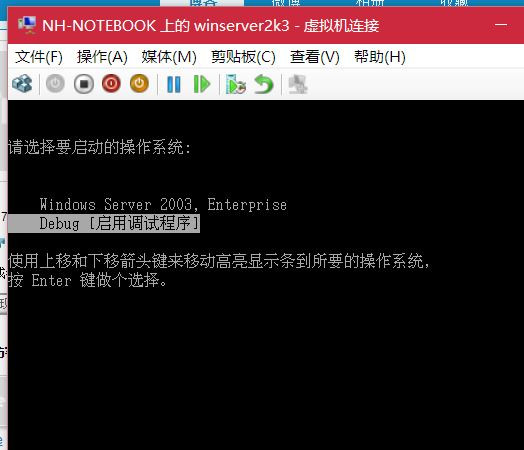
\includegraphics[width=0.4\textwidth]{2.jpg}\\
    \caption{boot选项\label{boot}}
\end{figure}

\begin{figure}
    \centering
    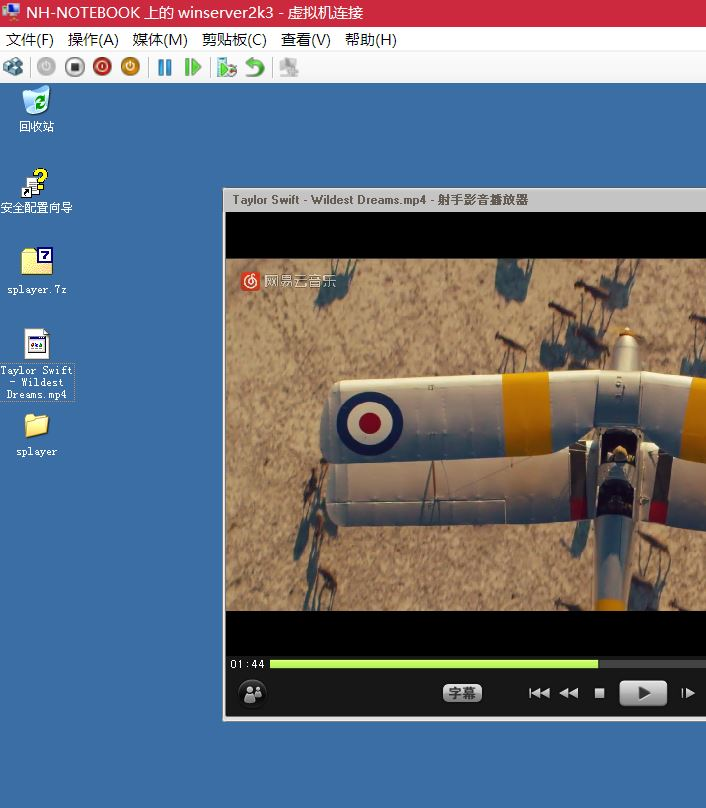
\includegraphics[width=0.4\textwidth]{1.jpg}\\
    \caption{正常工作\label{video}}
\end{figure}

\section{实验感想}
本实验一开始思考比较简单,因为无论是WRK还是Linux内核都有着大量的资料,而且本实验的目的是一致,只需要利用原有的接口进行一定的修改即可。

但是随着任务的深入,很多问题并不如想象的顺利:linux在3.x版本起对红黑树部分进行了大改,原有文档过于陈旧;系统接口难以的定位;MS的symbol服务器关机导致WinDbg难以进行复杂调试;两者数据结构差异而导致的算法细节区别较大;联合体这一少见数据结构的陷阱。

这一个个问题很令我烦恼,也消耗了大量的时间在其中去解决,但我从中学到了很多。我学会了更好的利用ctag去阅读代码,学会了更好的从大量资料中去寻找信息,学会了将大型项目中的函数及其依赖剥离出来进行测试\footnote{见测试文件中的测试项目},了解了Linux内核和Windows内核迥异的代码风格以及他们在虚拟内存管上的异同,对操作系统有了更深一步的理解。

虽然本次实验所涉及的VAD修改只是操作系统的一小部分,它仅仅完成是内存的组织、分配、调度和回收,但这一过程除去了操作系统的神秘感,使我能更好的去探索这两份代码中的秘密,也为以后的学习工作带来很好的基础。
\section{实验代码}
系统原有代码见origin文件夹,修改后的部分都存储在addrsup.c文件中,使用时直接用addrsup.c替换wrk中的同名文件编译即可。
\lstinputlisting{addrsup.c}
\end{document}
